\documentclass[10pt,mathserif]{beamer}
\usetheme{Dresden}

\usepackage{graphicx,amsmath,amssymb,tikz,psfrag}
\input defs.tex
\setbeamertemplate{blocks}[rounded][shadow]
\usepackage{yfonts}
\usepackage{booktabs}% http://ctan.org/pkg/booktabs
%% formatting
\usepackage{tcolorbox}

\mode<presentation>
{
	\usetheme{default}
}
\setbeamertemplate{navigation symbols}{}
\usecolortheme[rgb={0.13,0.28,0.59}]{structure}
\setbeamertemplate{itemize subitem}{--}
\setbeamertemplate{frametitle} {
	\begin{center}
		{\large\bf \insertframetitle}
	\end{center}
}

\newcommand\footlineon{
	\setbeamertemplate{footline} {
		\begin{beamercolorbox}[ht=2.5ex,dp=1.125ex,leftskip=.8cm,rightskip=.6cm]{structure}
			\footnotesize \insertsection
			\hfill
			{\insertframenumber}
		\end{beamercolorbox}
		\vskip 0.45cm
	}
}
\footlineon

\AtBeginSection[] 
{ 
	\begin{frame}<beamer> 
		\frametitle{Outline} 
		\tableofcontents[currentsection,currentsubsection] 
	\end{frame} 
} 

%% begin presentation

\title{\large \bfseries Mining the US Technologists Data}

\author{Abulitibu Tuguluke\\[3ex]
(Group 5)\\
	DHI Group Inc., CU Boulder}

\date{\today}

\begin{document}
	
	\frame{
		\thispagestyle{empty}
		\titlepage
	}
	

\section{Introduction} 
	\begin{frame}
	\frametitle{Before we start}
\begin{block}{}
\begin{itemize}
\item Why we choose to mine the technologist data?
 "by 2030, more than 85 million jobs could go unfilled because there are not enough skilled people to take them, according to the latest study conducted by Korn Ferry.
\item What is a  'Technologist'?
The simplest definition of a technologist is an expert in a particular field of technology. 
\item What is a 'Skill set'?
As the name suggests, it is the skill that associate with job title of a candidate. Although a individual, such as myself, would like to fit everything single skill that she has ever grasped into a resume, we only consider certain words that are associated with the job title.
\end{itemize}
\end{block}
\end{frame}
\section{Previous/Related Work}
	\begin{frame}
	\frametitle{SpaCy POS}
{
	\begin{center}
		\begin{tabular}{| l | l | l | l | l | r| } 
			\hline
			&	Sentence	&	Word	&	Tag	 & POS &	Job description \# \\ \hline
			0	&	1	&	Softwares		&Tech	& NNPS	&description: 1 \\ \hline
			1	&	2	&	SQL	&	Tech	& NNP &	description: 1 \\ \hline
			2	&	3	&	Java	&	Tech & NNPJ	&	description: 1	\\ \hline
			3		&4		&Web	&	Tech	& NNS&	description: 1\\ \hline
			4	&	5	&	Azure		&Tech	& NNP	&description: 1\\ \hline
			\vdots	&		\vdots	&		\vdots		&	\vdots	&	\vdots	&	\vdots\\ \hline
		\end{tabular}
\end{center}}

\end{frame}

	\begin{frame}
	\frametitle{Algo}

\begin{center}
	\begin{tabular}{ | p{2.5cm} |p{4.5cm} |}
		\hline
		Job & Skills \\ \hline
		Net Application Developer& Microsoft technologies;Software development;C$\#$;HTML;Quality assurance;ASP.NET;Visual Basic .NET;.NET;Agile.\\\hline
		Android Developer	& Software development;Java;Mobile development;Quality assurance;Android development.\\\hline
		\vdots	&	\vdots\\ \hline
	\end{tabular}
\end{center}
	
\end{frame}


\section{Data Set}
	\begin{frame}
	\frametitle{U.S. Department of Labor data}
	
	\begin{table}[h!]
		\caption{Deparrtment of  labour data }
		\resizebox{\columnwidth}{!}
		{%
			
			\begin{tabular}{llll}
				\hline
				{} &    count &  unique &                     top \\
				\hline
				occ\_code   &    14027 &    1507 &                 29-2010 \\
				occ\_group  &     9731 &       5 &                detailed \\
				occ\_title  &    14027 &    1272 &  Tour and Travel Guides \\
				group      &       46 &       2 &                   major \\
				tot\_emp    &  14027.0 &  8936.0 &                 11860.0 \\
				annual     &      852 &       1 &                    True \\
				hourly     &       62 &       1 &                    True \\
				year       &  14027.0 &     NaN &                     NaN \\
				area       &   2658.0 &     NaN &                     NaN \\
				\hline
			\end{tabular}
			
		}
	\end{table}
\end{frame}
	\begin{frame}
	\frametitle{U.S. Department of Labor data}
	\begin{figure}[h]
		\begin{center}
			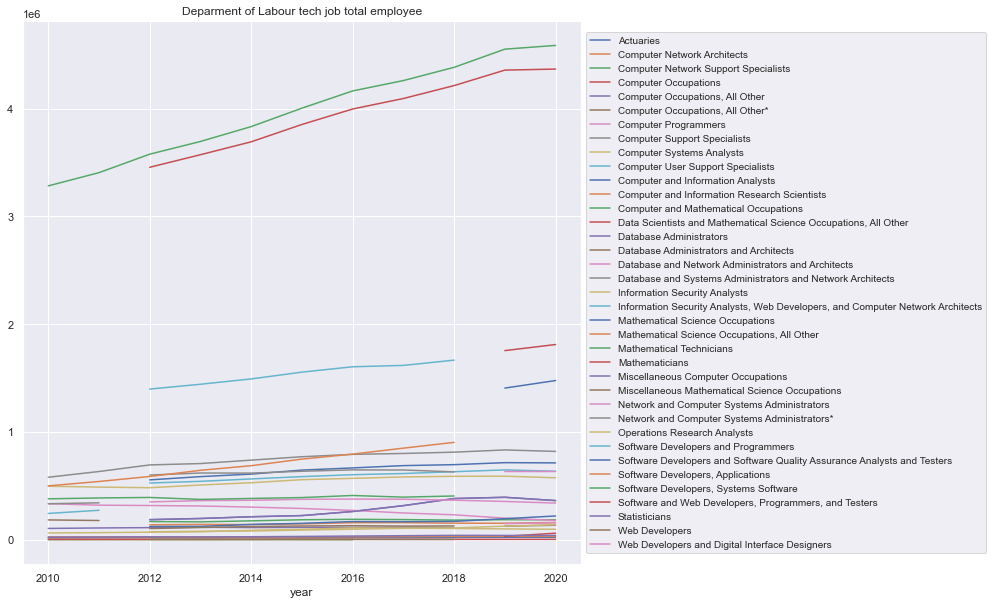
\includegraphics[width=\linewidth]{./photos/totaltech.png}
		\end{center}
		\caption{Deparment of Labour tech jobs number of employee.}
		\label{dolnumofemployee}
	\end{figure}
\end{frame}

	\begin{frame}
	\frametitle{U.S. Department of Labor data}
\begin{figure}[h]
	\begin{center}
		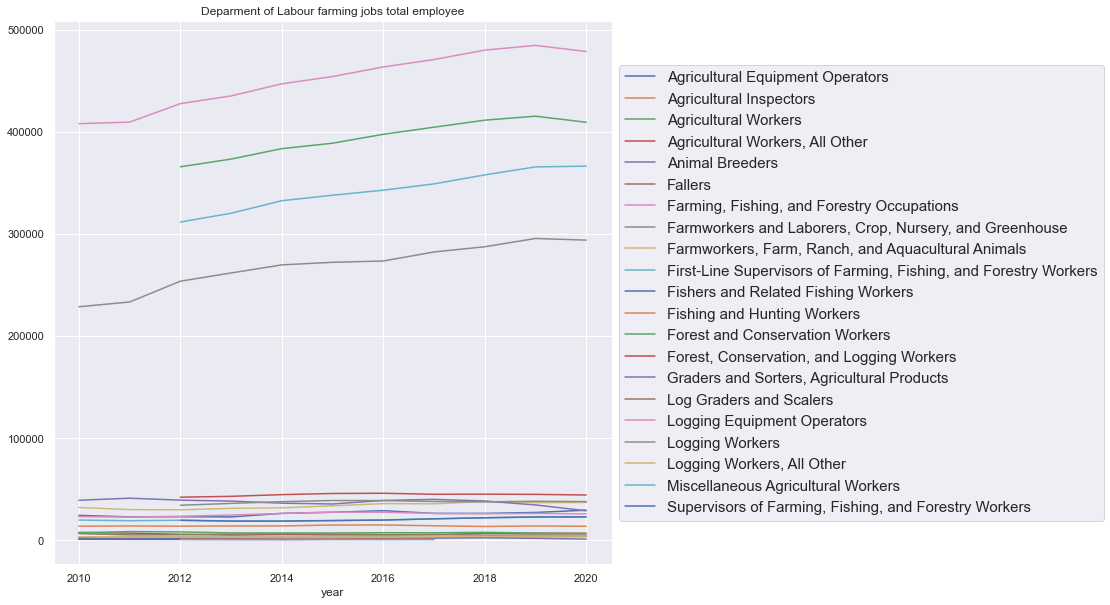
\includegraphics[width=\linewidth]{./photos/dolfarming.png}
	\end{center}
	\caption{Deparment of Labour farming jobs number of employee.}
	\label{dolfarming}
\end{figure}
\end{frame}

	\begin{frame}
	\frametitle{U.S. Department of Labor data}
\begin{figure}[h]
	\begin{center}
		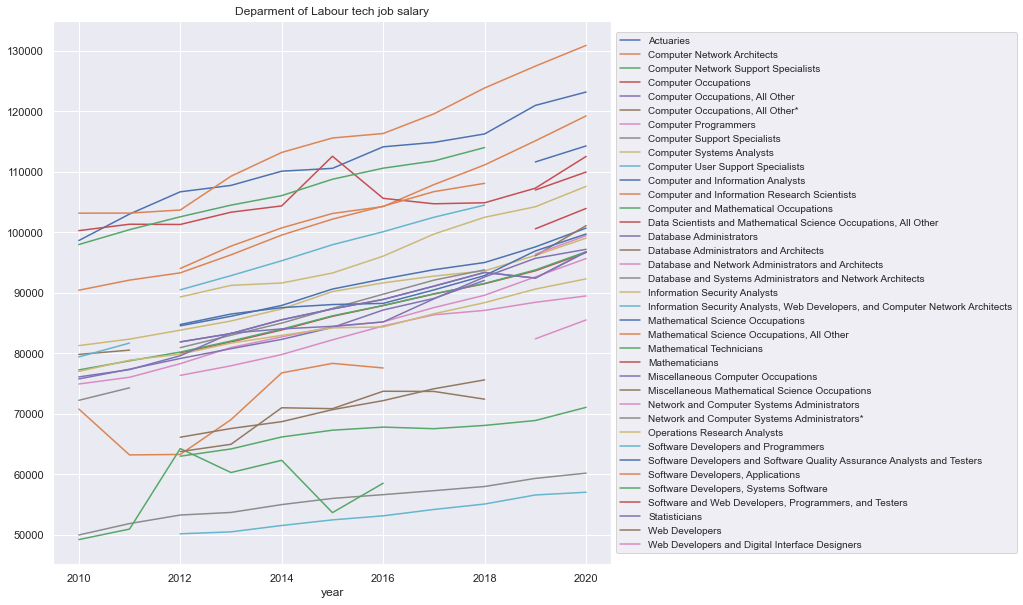
\includegraphics[width=\linewidth]{./photos/departmentoflabour.png}
	\end{center}
	\caption{Deparment of Labour tech job salary.}
	\label{techsalary}
\end{figure}
\end{frame}


	\begin{frame}
	\frametitle{H1b data}
	\begin{table}[h]
	\caption{Scrapped data as off July 15th}
	\resizebox{\columnwidth}{!}
	{%
		\begin{tabular}{lllll}
			\hline
			{} &    count & unique &                                                top &    freq \\
			\hline
			Dice\_job\_title &  2495079 &   1180 &                                    Systems Analyst &  198860 \\
			EMPLOYER       &  2495052 &  66795 &                  TATA CONSULTANCY SERVICES LIMITED &  157580 \\
			JOB TITLE      &  2467304 &   1770 &                                    SYSTEMS ANALYST &  198719 \\
			BASE SALARY    &  2467304 &  37871 &                                             60,000 &  146505 \\
			LOCATION       &  2467304 &  10474 &                                       NEW YORK, NY &  136642 \\
			SUBMIT DATE    &  2467304 &   2749 &                                         03/13/2015 &   14268 \\
			START DATE     &  2467304 &   2898 &                                         09/01/2015 &   32532 \\
			Job\_Title      &  2495079 &   1180 &                                    Systems Analyst &  198860 \\
			%		relatedSkills  &  2489574 &   1101 &  Software development;Systems analysis;SQL;Qual... &  198860 \\
			\hline
		\end{tabular}
	}
\end{table}

\end{frame}
	\begin{frame}
	\frametitle{EDA}
\begin{figure}[h]
	
	\centering
	\begin{minipage}{.48\linewidth}
		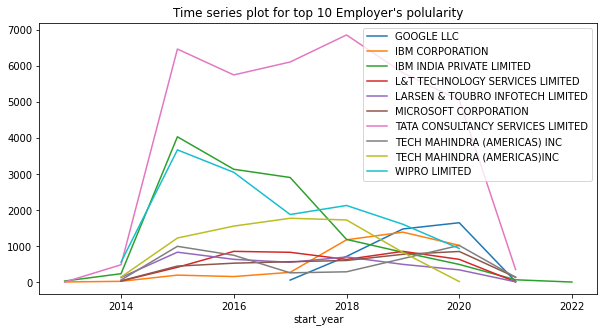
\includegraphics[width=\linewidth]{./photos/top10employers_timeseries.png}
		
		
	\end{minipage}
	\hfill
	\begin{minipage}{.48\linewidth}
		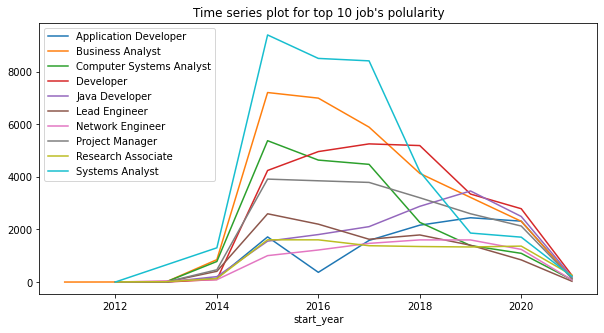
\includegraphics[width=\linewidth]{./photos/top10job_timeseries.png}
		
		
	\end{minipage}
	\caption{Top 10 employers and top 10 jobs.}
	\label{leastpopular}
\end{figure}
\end{frame}

	\begin{frame}
	\frametitle{EDA}
	\begin{figure}[h]
		
		\centering
		\begin{minipage}{.48\linewidth}
			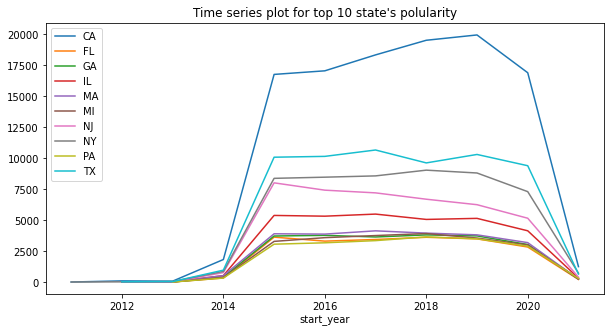
\includegraphics[width=\linewidth]{./photos/top10state_timeseries.png}
			
			
		\end{minipage}
		\hfill
		\begin{minipage}{.48\linewidth}
			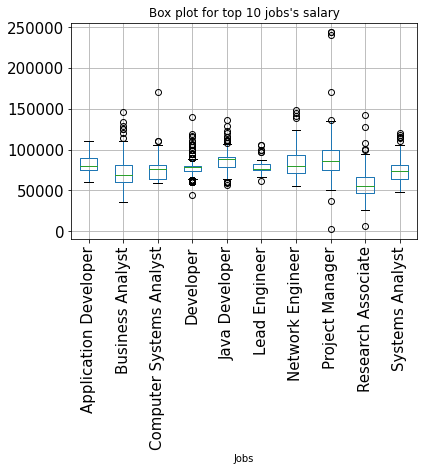
\includegraphics[width=.7\linewidth]{./photos/top10jobs.png}
			
			
		\end{minipage}
		\caption{Top 10 states and top 10 jobs salary.}

	\end{figure}
\end{frame}

	
\section{Main Techniques Applied}
	\begin{frame}
	\frametitle{Data cleaning}
\begin{table}[h!]
	\caption{New h1b data after data cleaning process}
	\label{newdata}
	\resizebox{\columnwidth}{!}
	{%
		
		\begin{tabular}{lllll}
			\hline
			{} &   count & unique &                                                top &   freq \\
			\hline
			Dice\_job\_title &  603967 &   1107 &                                    Systems Analyst &  35605 \\
			EMPLOYER       &  603967 &  66538 &                  TATA CONSULTANCY SERVICES LIMITED &  36885 \\
			JOB TITLE      &  603967 &   1655 &                                    SYSTEMS ANALYST &  35605 \\
			BASE SALARY    &  603967 &  37791 &                                             60,000 &  23256 \\
			LOCATION       &  603967 &  10453 &                                       NEW YORK, NY &  34957 \\
			SUBMIT DATE    &  603967 &   2747 &                                         03/16/2018 &   2377 \\
			START DATE     &  603967 &   2897 &                                         10/01/2020 &  17065 \\
			Job\_Title      &  603967 &   1107 &                                    Systems Analyst &  35605 \\
			%			relatedSkills  &  603967 &   1101 &  Software development;Systems analysis;SQL;Qual... &  35605 \\
			\hline
		\end{tabular}
		
	}
	
\end{table}
\end{frame}
	\begin{frame}
	\frametitle{K-Mean}
	\begin{figure}[h]
	
	\centering
	\begin{minipage}{.48\linewidth}
		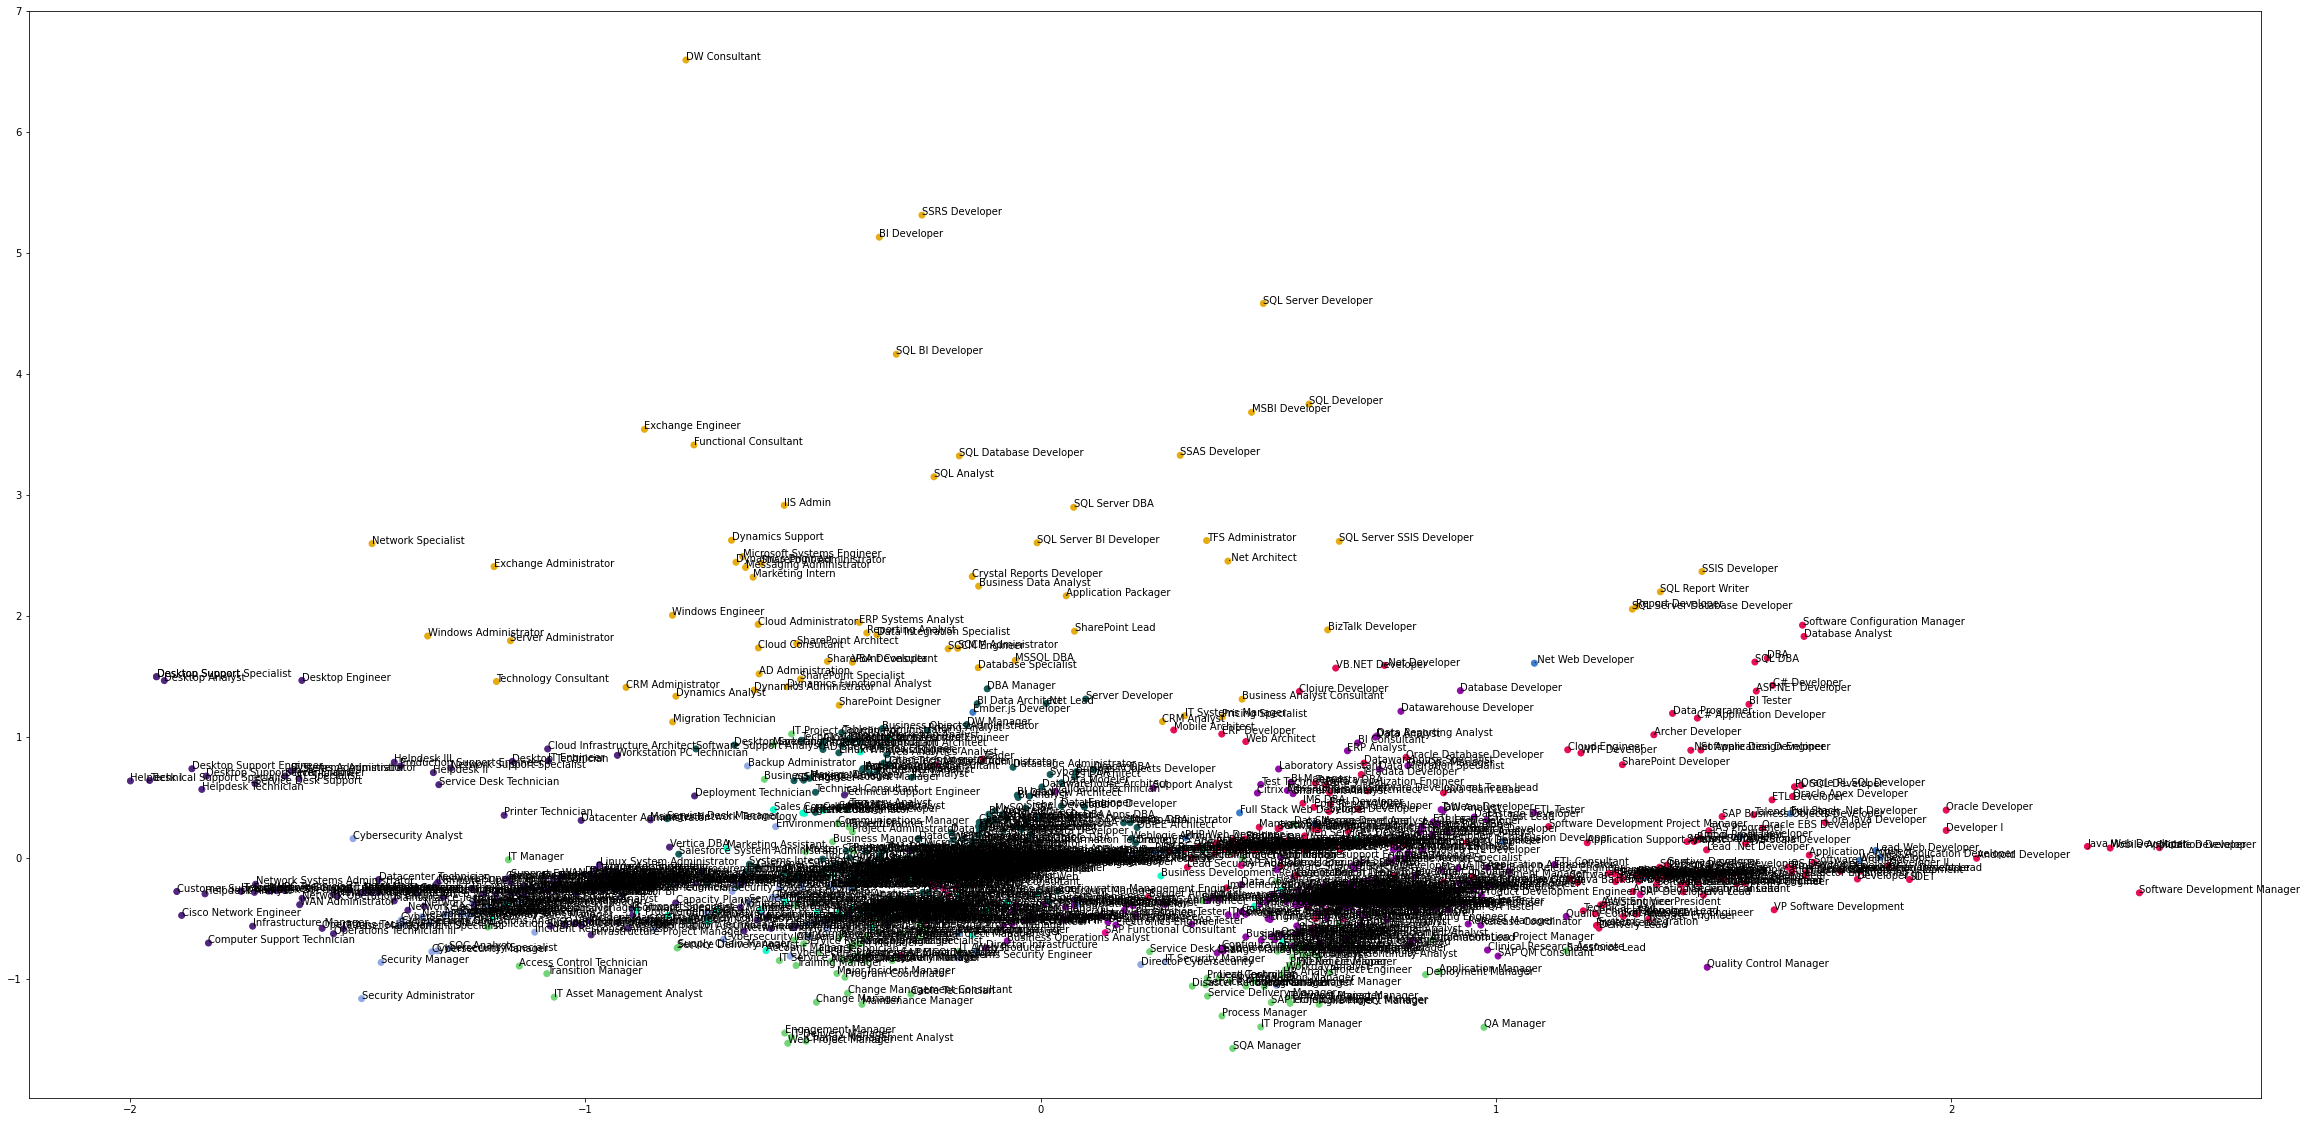
\includegraphics[width=\linewidth]{./photos/clusterscatter.png}
		
		
	\end{minipage}
	\hfill
	\begin{minipage}{.48\linewidth}
		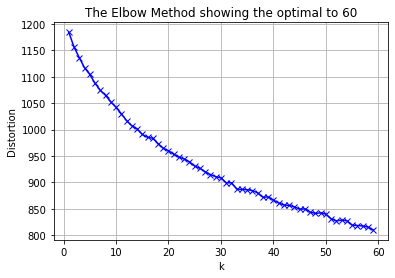
\includegraphics[width=.7\linewidth]{./photos/elbow.png}
		
		
	\end{minipage}
	\caption{PCA + K-mean + Elbow.}
	
\end{figure}
\end{frame}


\section{Key Results}
	\begin{frame}
	\frametitle{Trending Skills}
\begin{figure}[h]
	\begin{center}
		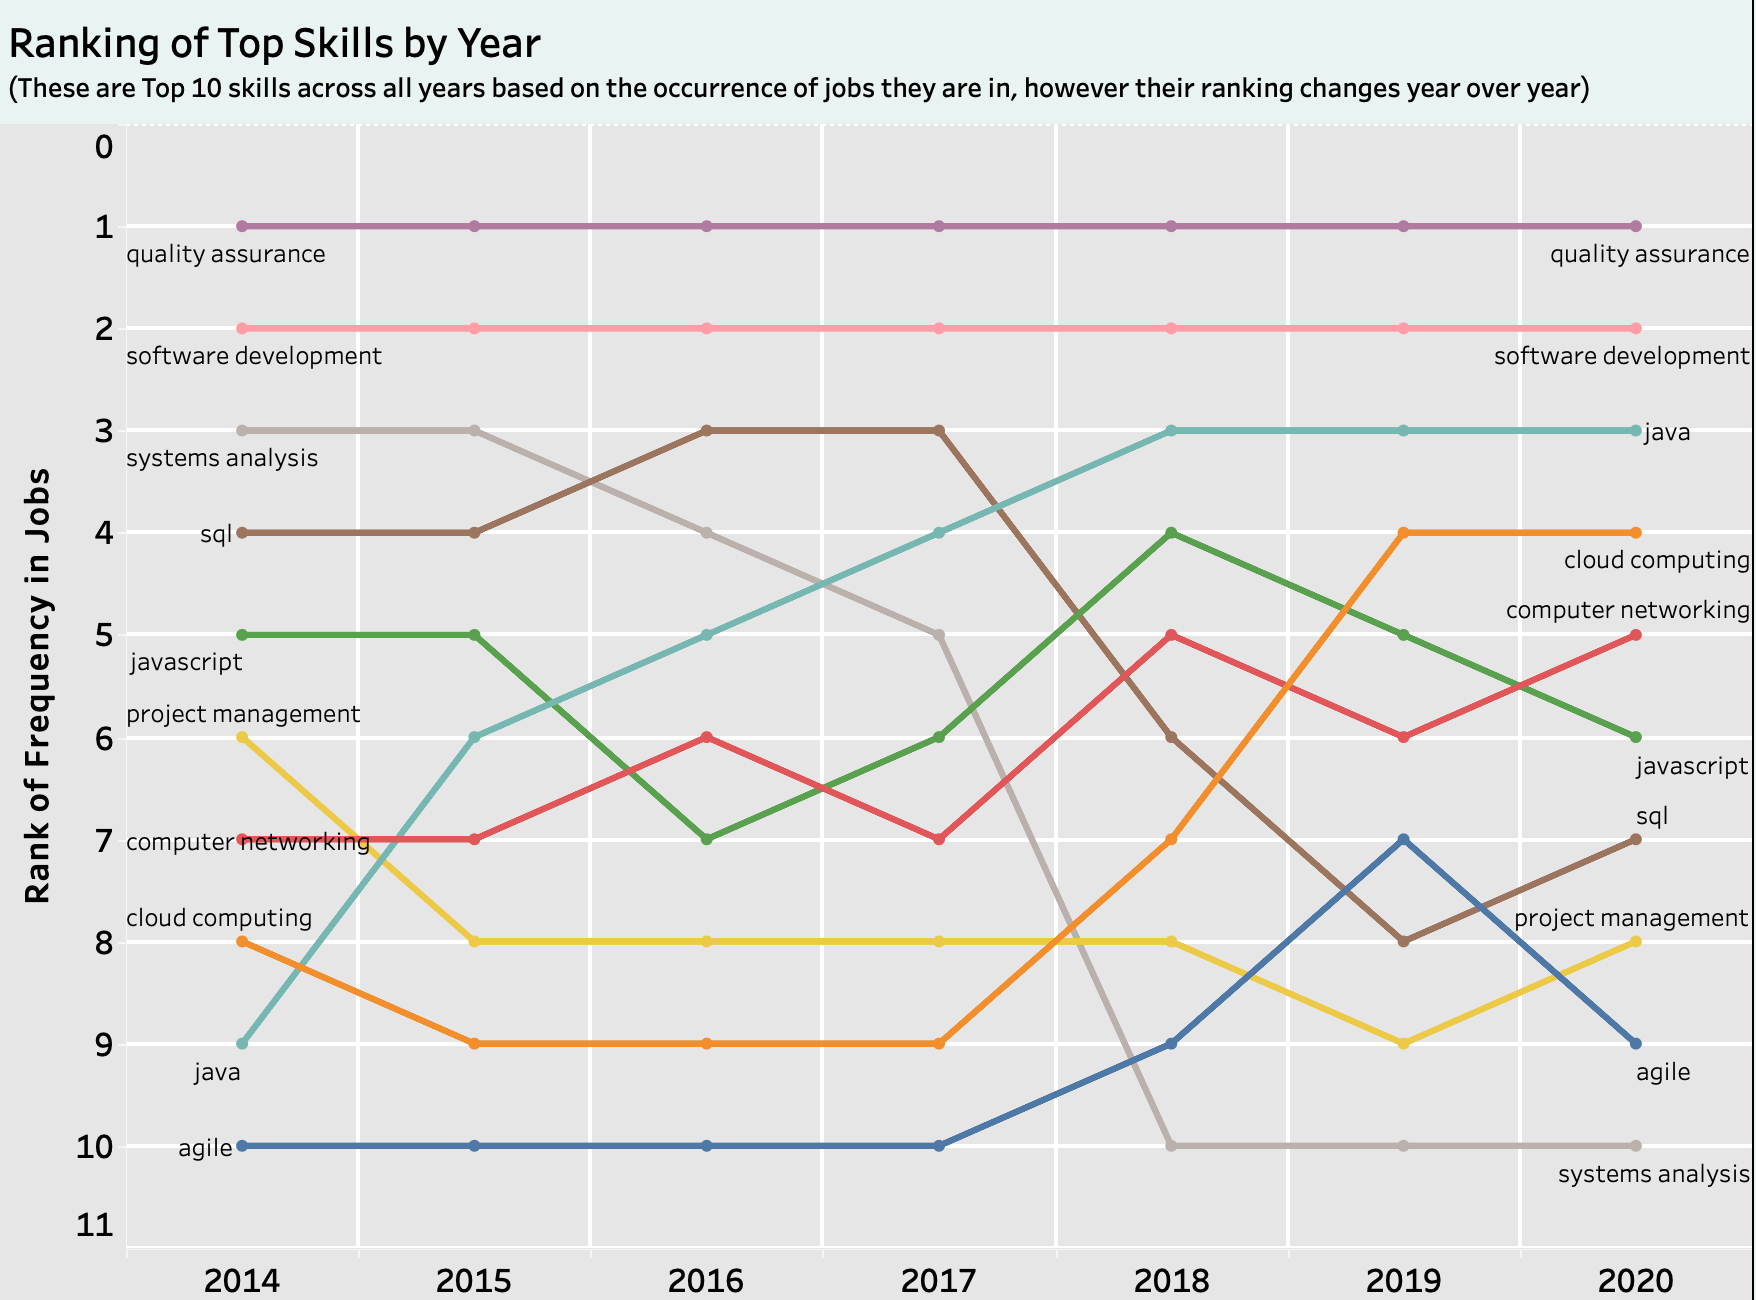
\includegraphics[width=.8\linewidth]{./photos/top10 ranking.png}
	\end{center}
	\caption{Skill 'trendiness' throughout the years}
	\label{trending}
\end{figure}

\end{frame}

	\begin{frame}
	\frametitle{clustering}
	\begin{itemize}
	\item Cluster 0
	sap	

	sap fi	
	sap fico	
	sap grc	
	sap mm

	sap pp	
	\item Cluster 1
	data warehouse	
	database
	etl	
	microsoft sql server
	microsoft ssis	
	quality assurance	
	software developmen
	sql
\end{itemize}	
We can easily guess that cluster 0 is SAP related, 1 is database. 2 is cyber-security, 4 is marketing, 5 is web developer, 7 computer is hardware, 8 is project management, 9 is software engineering.\\
Only cluster 3(health-tech) and 6 (Fin-tech) are a bit hard to define. Overall results for unsupervised learning is beyond our early expectation.
\end{frame}
\section{Applications}	

	\begin{frame}
	\frametitle{Application}
There are infinite fields that our knowledge gain from this project be applied to. First, is the bigger picture of technology demand in  the US. For any recruiting company, the huge demand of particular job titles are the first thing they should pay attention to, since it is consider the 21st century capital, and need to competed for.\\
Second is for job market on which skill-sets are in need so that job-seekers can have a better vision. Words like `A.I.' and `Machine learning' are too vague to be focused on, while skill-set from our cluster study shows that:\\
Third, there can be a better job category mapping within the knowledge gained, how and why certain jobs should be labeled as the same title with text clustering and Fuzzy matching. 
Many applications can be achieved with the future work on the same topic, due to the time limit for this project, we will sketch out the big picture for the future study in the next section. 
	
\end{frame}
\section{Future work}
	\begin{frame}
	\frametitle{Knowledge graph}
	\begin{figure}[h]
		
		\centering
		\begin{minipage}{.48\linewidth}
			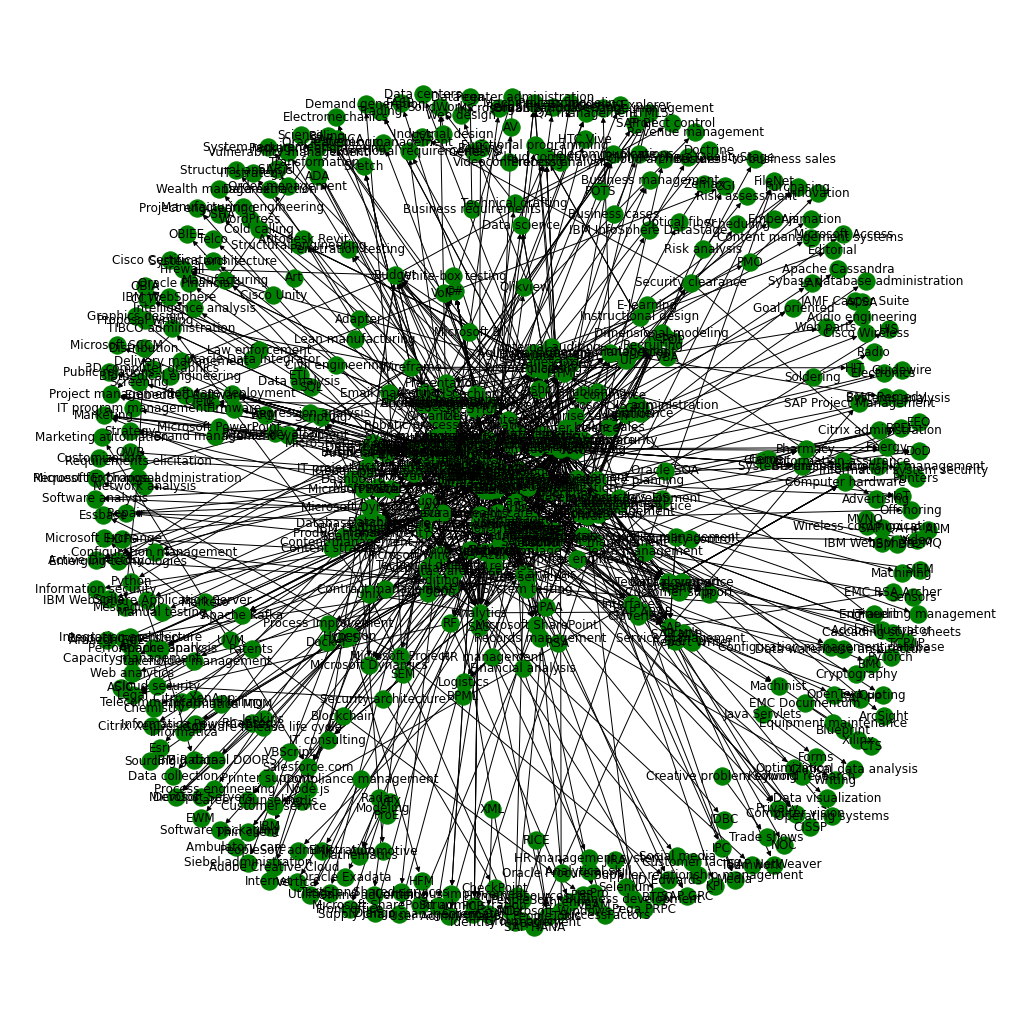
\includegraphics[width=\linewidth]{./photos/knowlegegraphsmall.png}
			
			
		\end{minipage}
		\hfill
		\begin{minipage}{.48\linewidth}
			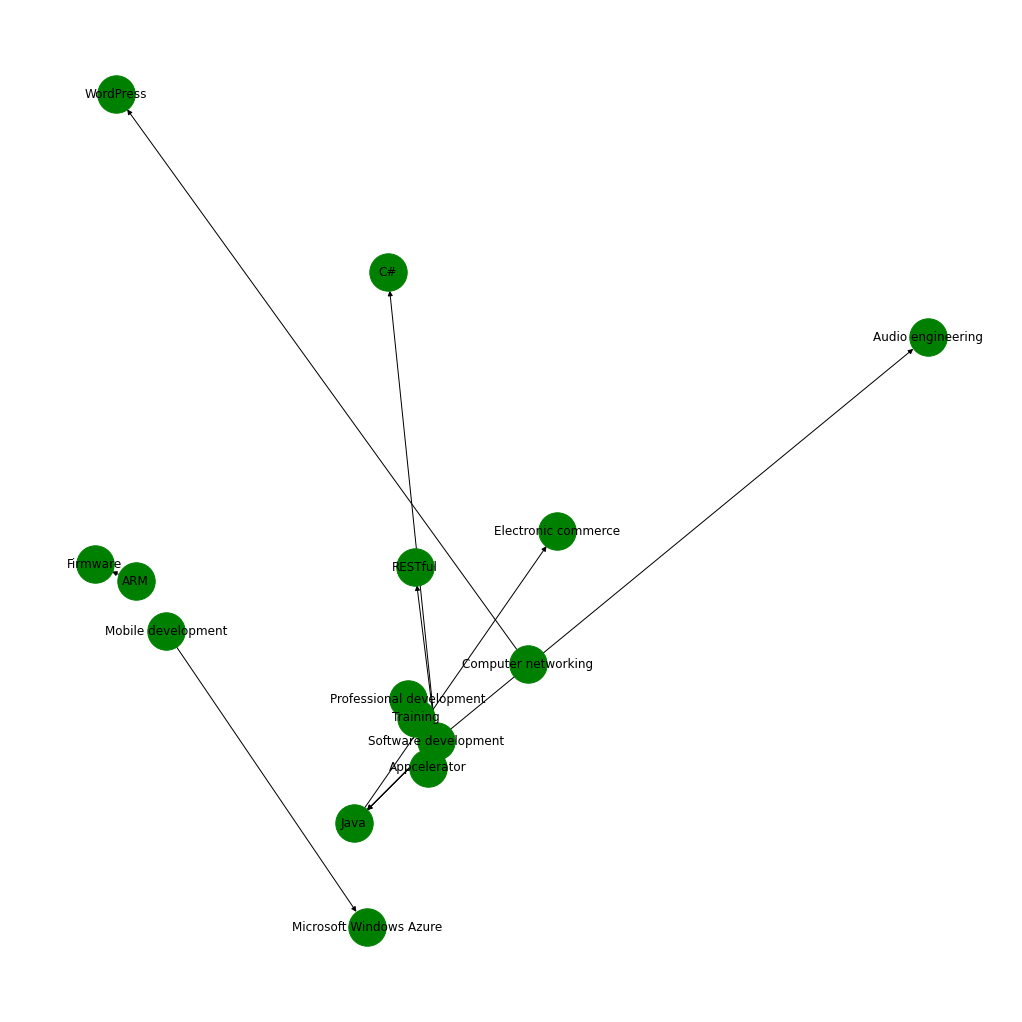
\includegraphics[width=.7\linewidth]{./photos/knowledgearrow2.png}
			
			
		\end{minipage}
		\caption{knowledge arrow}
		
	\end{figure}
MORE DATA. FROM SUPPLY SIDE 
\end{frame}

\section{Conclusion}
	\begin{frame}
	\frametitle{What did we do and learn?}
	\tiny
In this project, we study the mining of US technologist data by combining US department of labor data along with web scraped H1b data set, after the introduction of word tagging to get skill set data, we clean and analyze the processed and joined data to later clustering the job skill data set. Since there is no clear technologist mining or analysis report online, our objective is to fill the blank page with knowledge of technologist's trench in the US studying  time series and Geo data. Our study shows that on top of tech talent demand in US are on the rise, is cloud engineering and project management skills will be in huge demand, while SQL and system analysis are in decline. Java still grows strong as python has not yet replace its spot, and Software developers should not worry that data scientists or ML engineers will make their job obsolete. \\
Our study's limitation is the availability of  lasted H1b data set along with non guidance on job title mapping table. In the first case: we are not able to do a deep time series analysis and prediction, in the latter, we do not have optimal clustering number for the unsupervised learning. 
We are looking forward to the future development of this topic with a better data set collection, the study of each topic can be its own project: Knowledge graph for each skill set, supply and demand of each job tile in the US hiring market, semi-supervised clustering with title mapping, and dynamic prediction for each skill and title.
	
\end{frame}
\section{Visualization}
	\begin{frame}
	\frametitle{Application}
\url{https://public.tableau.com/app/profile/abulitibu.tuguluke/viz/H1BApplicationsv2/H1BJobs?publish=yes}
\end{frame}


	\begin{frame}
	\frametitle{}
	\centering
	\huge
Questions?
\end{frame}


	\begin{frame}
	\frametitle{}
	\centering
	\huge
Thank you
\end{frame}
\end{document}